\subsection{Geluid en licht}

\subsubsection{Gedrag}
Op het LCD is te zien of het geluid en/of het licht aangaat als het alarm afgaat. Dit is optioneel en kan geregeld worden in het menu. Het signaal menu\_state geeft aan in welk deel van het menu de gebruiker zich bevindt.

\subsubsection{Functionaliteit}
De subblokken licht en geluid lijken veel op elkaar. In figuren \ref{fig:FSMgeluid} en \ref{fig:FSMlicht} zijn de FSM van de twee blokken te zien.

\subsubsection{FSM}

\begin{figure}[h!]
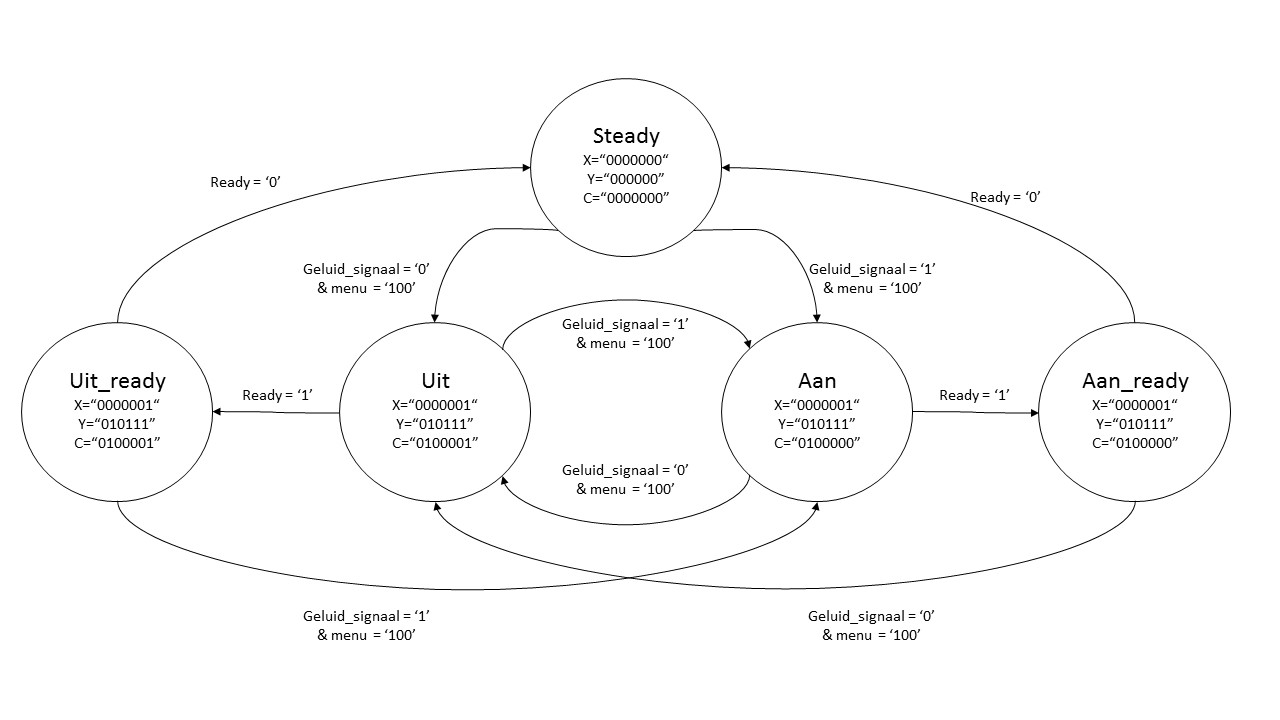
\includegraphics[width=15cm]{verslagschemas/FSMs/geluid.jpg}
\caption{FSM van het subblok geluid}
\label{fig:FSMgeluid}
\end{figure}

\begin{figure}[h!]
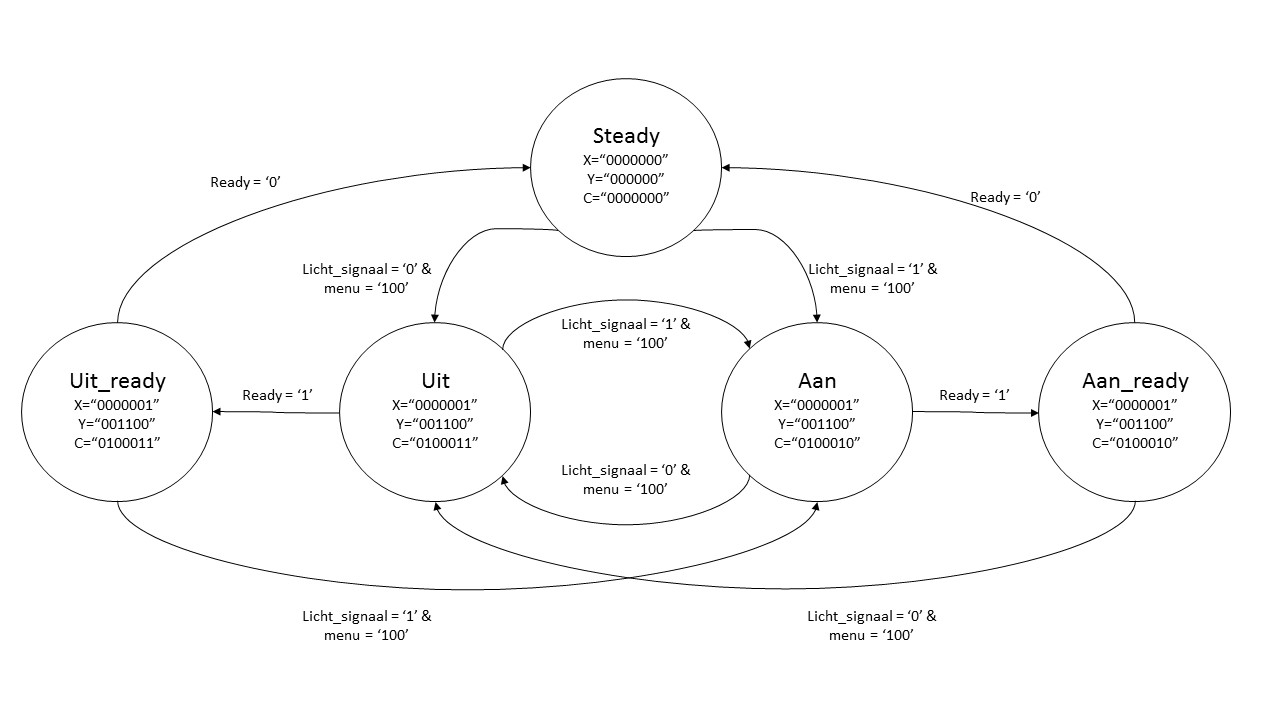
\includegraphics[width=15cm]{verslagschemas/FSMs/licht.jpg}
\caption{FSM van het subblok licht}
\label{fig:FSMlicht}
\end{figure}

\subsubsection{VHDL code}

\subsubsection{Simulaties}
In appendix \ref{Ap:sim_LCD} zijn de resultaten te zien van de subblokken \it{geluid} en \it{licht}.

\subsubsection{Testen}

\subsubsection{Resultaten}

\subsubsection{Discussie}